\documentclass[12pt,oneside,a4paper]{article}
\usepackage[utf8]{inputenc}
\usepackage[brazil]{babel}

\usepackage{settings/preambule}

\usepackage{listings}

\definecolor{codegreen}{rgb}{0,0.6,0}
\definecolor{codegray}{rgb}{0.5,0.5,0.5}
\definecolor{codepurple}{rgb}{0.58,0,0.82}
\definecolor{backcolour}{rgb}{0.95,0.95,0.92}

\lstdefinestyle{mystyle}{
    language=Scilab,
    backgroundcolor=\color{backcolour},   
    commentstyle=\color{codegreen},
    keywordstyle=\color{magenta},
    numberstyle=\tiny\color{codegray},
    stringstyle=\color{codepurple},
    basicstyle=\ttfamily\footnotesize,
    breakatwhitespace=false,         
    breaklines=true,                 
    captionpos=b,                    
    keepspaces=true,                 
    numbers=left,                    
    numbersep=5pt,                  
    showspaces=false,                
    showstringspaces=false,
    showtabs=false,                  
    tabsize=2,
    literate      =        % Support additional characters
      {á}{{\'a}}1  {é}{{\'e}}1  {í}{{\'i}}1 {ó}{{\'o}}1  {ú}{{\'u}}1
      {Á}{{\'A}}1  {É}{{\'E}}1  {Í}{{\'I}}1 {Ó}{{\'O}}1  {Ú}{{\'U}}1
      {à}{{\`a}}1  {è}{{\`e}}1  {ì}{{\`i}}1 {ò}{{\`o}}1  {ù}{{\`u}}1
      {À}{{\`A}}1  {È}{{\'E}}1  {Ì}{{\`I}}1 {Ò}{{\`O}}1  {Ù}{{\`U}}1
      {ä}{{\"a}}1  {ë}{{\"e}}1  {ï}{{\"i}}1 {ö}{{\"o}}1  {ü}{{\"u}}1
      {Ä}{{\"A}}1  {Ë}{{\"E}}1  {Ï}{{\"I}}1 {Ö}{{\"O}}1  {Ü}{{\"U}}1
      {â}{{\^a}}1  {ê}{{\^e}}1  {î}{{\^i}}1 {ô}{{\^o}}1  {û}{{\^u}}1
      {Â}{{\^A}}1  {Ê}{{\^E}}1  {Î}{{\^I}}1 {Ô}{{\^O}}1  {Û}{{\^U}}1
      {œ}{{\oe}}1  {Œ}{{\OE}}1  {æ}{{\ae}}1 {Æ}{{\AE}}1  {ß}{{\ss}}1
      {ç}{{\c c}}1 {Ç}{{\c C}}1 {ø}{{\o}}1  {å}{{\r a}}1 {Å}{{\r A}}1
      {ã}{{\~a}}1  {õ}{{\~o}}1  {Ã}{{\~A}}1 {Õ}{{\~O}}1
      {ñ}{{\~n}}1  {Ñ}{{\~N}}1  {¿}{{?`}}1  {¡}{{!`}}1
      {°}{{\textdegree}}1 {º}{{\textordmasculine}}1 {ª}{{\textordfeminine}}1
      % ¿ and ¡ are not correctly displayed if inconsolata font is used
      % together with the lstlisting environment. Consider typing code in
      % external files and using \lstinputlisting to display them instead. 
}

\lstset{style=mystyle}

\usepackage{listings}

%\definecolor{codegreen}{rgb}{0,0.6,0}
\definecolor{codegreen}{RGB}{100,174,100}
\definecolor{codegray}{rgb}{0.5,0.5,0.5}
\definecolor{codepurple}{rgb}{0.58,0,0.82}
\definecolor{backcolour}{rgb}{0.95,0.95,0.92}
%\definecolor{backcolour}{RGB}{247,247,242}
%\definecolor{backcolour}{RGB}{252, 252, 247}

\definecolor{codeblue}{RGB}{50,185,185}
\definecolor{stringcolor}{RGB}{188,143,143}
\definecolor{emphcolor}{RGB}{176,24,19}
\definecolor{conditional}{RGB}{160,32,240}
\definecolor{variables}{RGB}{131,67,16}
\definecolor{brackets}{RGB}{74,85,219}
\definecolor{stops}{RGB}{95,158,160}
\definecolor{infinity}{RGB}{218,112,214}
\definecolor{operators}{RGB}{92,92,92}
\definecolor{colon}{RGB}{255,170,0}

\renewcommand{\ttdefault}{pcr}

\lstdefinestyle{scilab_colors}{
    language=Scilab,
    %frame=single,
    backgroundcolor=\color{backcolour},   
    commentstyle=\color{codegreen},
    %keywordstyle=\color{magenta},
    keywordstyle=\color{codeblue},
    numberstyle=\tiny\color{codegray},
    %identifierstyle=\color{blue},
    %stringstyle=\color{codepurple},
    stringstyle=\color{stringcolor},
    basicstyle=\ttfamily\footnotesize,
    emph={function,endfunction},
    emphstyle=\color{emphcolor},
    emph={[2]for, while, if, then, end},
    emphstyle={[2]\color{conditional}},
    emph={[3]lambda, x1, k, n_erro, A, x0, epsilon, alpha, M},
    emphstyle={[3]\bfseries\color{variables}}, 
    emph={[4]\$},
    emphstyle={[4]\color{colon}},
    emph={[5]Metodo_Potencia, Metodo_Potencia_2, Potencia_deslocada_inversa, Potencia_deslocada_Rayleigh},
    emphstyle={[5]\underbar},
    emph={[6]break, continue, return},
    emphstyle={[6]\color{stops}},
    emph={[7]\%inf},
    emphstyle={[7]\color{infinity}},
    emph={[8]Resolve_com_LU},
    emphstyle={[8]\bfseries\color{codepurple}},
    breakatwhitespace=false,         
    breaklines=true,                 
    captionpos=b,                    
    keepspaces=true,                 
    numbers=left,                    
    numbersep=5pt,                  
    showspaces=false,                
    showstringspaces=false,
    showtabs=false,                  
    tabsize=2,
    literate      =        % Support additional characters
      {á}{{\'a}}1  {é}{{\'e}}1  {í}{{\'i}}1 {ó}{{\'o}}1  {ú}{{\'u}}1
      {Á}{{\'A}}1  {É}{{\'E}}1  {Í}{{\'I}}1 {Ó}{{\'O}}1  {Ú}{{\'U}}1
      {à}{{\`a}}1  {è}{{\`e}}1  {ì}{{\`i}}1 {ò}{{\`o}}1  {ù}{{\`u}}1
      {À}{{\`A}}1  {È}{{\'E}}1  {Ì}{{\`I}}1 {Ò}{{\`O}}1  {Ù}{{\`U}}1
      {ä}{{\"a}}1  {ë}{{\"e}}1  {ï}{{\"i}}1 {ö}{{\"o}}1  {ü}{{\"u}}1
      {Ä}{{\"A}}1  {Ë}{{\"E}}1  {Ï}{{\"I}}1 {Ö}{{\"O}}1  {Ü}{{\"U}}1
      {â}{{\^a}}1  {ê}{{\^e}}1  {î}{{\^i}}1 {ô}{{\^o}}1  {û}{{\^u}}1
      {Â}{{\^A}}1  {Ê}{{\^E}}1  {Î}{{\^I}}1 {Ô}{{\^O}}1  {Û}{{\^U}}1
      {œ}{{\oe}}1  {Œ}{{\OE}}1  {æ}{{\ae}}1 {Æ}{{\AE}}1  {ß}{{\ss}}1
      {ç}{{\c c}}1 {Ç}{{\c C}}1 {ø}{{\o}}1  {å}{{\r a}}1 {Å}{{\r A}}1
      {ã}{{\~a}}1  {õ}{{\~o}}1  {Ã}{{\~A}}1 {Õ}{{\~O}}1
      {ñ}{{\~n}}1  {Ñ}{{\~N}}1  {¿}{{?`}}1  {¡}{{!`}}1 {[}{{\textcolor{brackets}{[}}}{1}
        {]}{{\textcolor{brackets}{]}}}{1}
        {(}{{\textcolor{brackets}{(}}}{1}
        {)}{{\textcolor{brackets}{)}}}{1} 
        {+}{{{\color{operators}+}}}1
        {-}{{{\color{operators}-}}}1
        {*}{{{\color{operators}*}}}1
        {/\ }{{{\color{operators}/}}}1
        {=}{{{\color{operators}=}}}1
        {^}{{{\color{operators}\textasciicircum}}}1
        {<}{{{\color{operators}<}}}1
        {>}{{{\color{operators}>}}}1
        %{&}{{{\color{operators}\&}}}1
        %{!=}{{{\color{codegreen}$\neq$}}}1
        %{~}{{{\color{operators}\textasciitilde}}}{1}
        %{:}{{{\color{colon}:}}}{1}
      {°}{{\textdegree}}1 {º}{{\textordmasculine}}1 {ª}{{\textordfeminine}}1
      % ¿ and ¡ are not correctly displayed if inconsolata font is used
      % together with the lstlisting environment. Consider typing code in
      % external files and using \lstinputlisting to display them instead.
}

%\lstset{style=scilab_colors}

\usepackage{etoolbox} % provides the \patchcmd macro
\makeatletter
\patchcmd{\lsthk@SelectCharTable}{`)}{``}{}{} % patch listings
%\patchcmd{\lsthk@SelectCharTable}{``}{`)}{}{} % undo patch if needed
\makeatother

\usepackage{hhline}

\newcommand{\fontcode}[2]{{\fontfamily{#1}\selectfont #2}}

%\title{Relatório - AP1_ALNum}
\title{Relatório\\Computação Escalável}
\student{Tiago da Silva \\João Alcindo Ribeiro de Azevedo\\Germano Andrade Brandão}
\local{Rio de Janeiro}

\coversheet{}%write 'yes' or left it blank

\professor{.}
\summary{.}

\begin{document}

\maketitle

\tableofcontents
\newpage


\section{Introdução}
    Trataremos aqui das decisões de projetos adotadas ao longo do trabalho, procurando esclarecer o nosso ponto de vista acerca de cada escolha. Além disso, toda a estrutura será detalhada, de forma a ser possível entender bem como funciona todo o processo de simulação de ponta a ponta. Por fim, mostraremos como o trabalho foi adaptado para que fosse processado em nuvem, utilizando majoritariamente os serviços da Amazon AWS.

\section{Pipeline}

	\begin{figure} 
		\centering 
		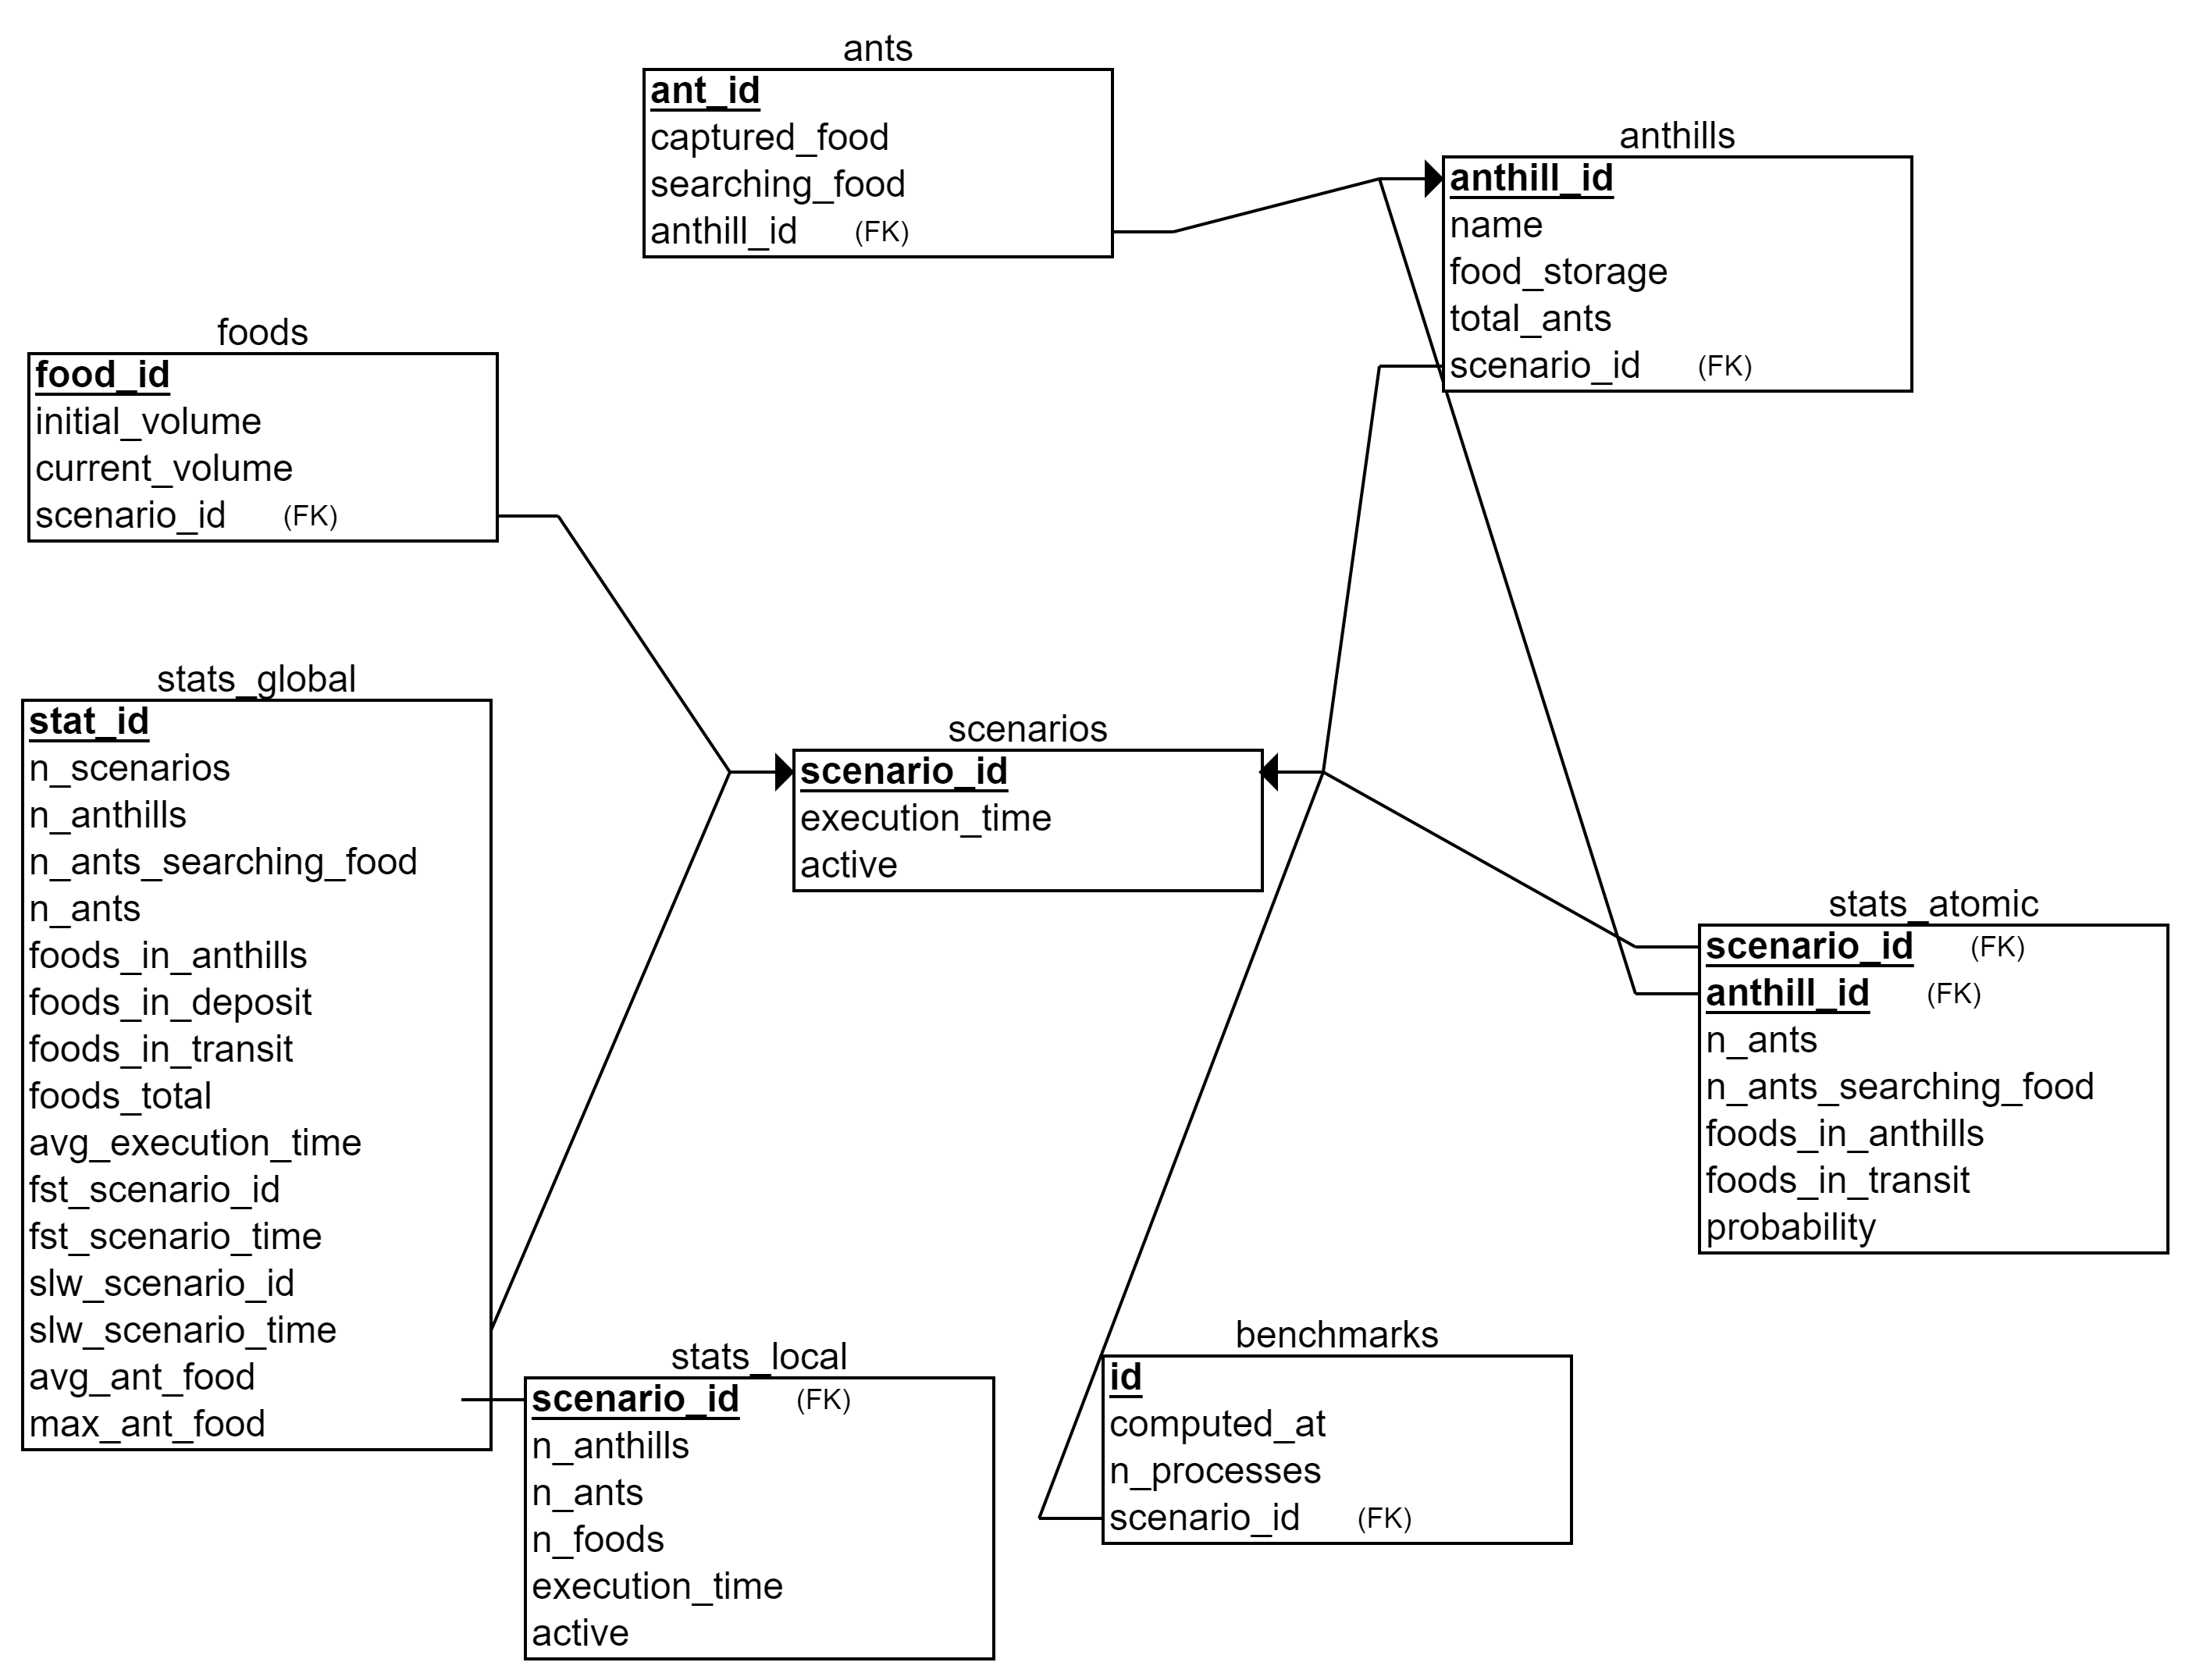
\includegraphics[width=\textwidth]{../images/relational_diagram.png} 
		\caption{Modelo relacional do banco de dados utilizado para a captura persistente dos dados gerados pela simulação.} 
		\label{fig:relational} 
	\end{figure} 

	Escolhemos uma pipeline de extração, transformação e carregamento (ETL, em oposição a ELT); importantemente, esta escolha está amarrada à contemplação de que os procedimentos para serializar os dados e os tornar receptivos a um banco de dados relacional gozam de intensidade computacinoal enxuta. Utilizamos, para isso, um banco de dados alicerçado no modelo relacional da Figura~\ref{fig:relational}. Nas seções seguintes, desta maneira, descrevemos a implementação de cada estágio de nosso pipeline ETL. 
	
	Neste ínterim, advogamos o modelo escolhido e apresentamos o framework geral para controlar a comunicação entre os processos responsáveis pelo inserção dos dados em um banco de dados. Inicialmente, as tabelas \texttt{scenarios}, \texttt{ants}, \texttt{anthills} e \texttt{foods} almejam incorporar as informações brutas geradas pelas simulações; isso enseja a expansão da amplitude de análises subsequentes. As tabelas com prefixo \texttt{stats\_}, por outro lado, são atualizadas periodicamente e permitem, desta maneira, o acesso, em diferentes aspectos de granularidades\footnote{Explicitamente, escrevemos \texttt{global} para as análises globais, que tangenciam todos os cenários executados; \texttt{local}, para as análises que consolidam os aspectos de cada cenário; e \texttt{atomic}, para as análises que conformam as instâncias que apontam para os formigueiros.}, às informações por usuários (na Seção~\ref{sec:user}, exploramos o desenho de uma interface que direciona o usuário ao exame dos cenários correntes e passados). Alternativamente, poderíamos 

	\begin{enumerate} 
		\item implementar uma base de dados analítica, com um modelo dimensional que combinasse parciomoniosamente as tabelas para o cômputo das quantidades solicitadas nos requisitos da modelagem;
		\item e, mais disruptivamente, optar pela utilização de um banco de dados noSQL, com um pipeline ELT, em que os dados seriam armazenados e, em seguida, processados. 
	\end{enumerate} 

	\noindent Nestas condições, nossas escolhas estão amarradas a compleições objetivas: com respeito a 1, precisaríamos comportar, em nosso sistema, um mecanismo de transferência de informações entre um banco de dados operacional e um analítico, trascendendo, em nossa opinião, o objetivo desta avaliação, que não inclui a modelagem dimensional; com respeito a 2, nossas breves exposições a bancos de dados noSQL (como o MongoDB) culminaram em nossas reticências em os introduzir neste sistema. Neste cenário, nossas escolhas por um banco de dados relacional estão alicerçadas em sua conveniência e na existência de múltiplas ferramentas que permitem a sua integração em um sistema distribuído. 

\subsection{Extração}
\subsection{Transformação}
\subsection{Carregamento}

\section{Armazenamento em nuvem (AWS)}
    O processamento e o armazenamento locais podem ser vantajosos por ter uma velocidade alta e não depender de conexões externas. No entanto, essas vantagens podem acabar rapidamente ao passo que a quantidade a ser processada/armazenada começa a aumentar. Nesse sentido, uma das alternativas mais adotadas atualmente é a de computação em nuvem, onde um ambiente vasto com soluções prontas ou customizáveis são disponibilizadas e de forma escalável, de acordo com a demanda.
    
    Dito isso, para esse trabalho utilizamos alguns dos serviços de nuvem da Amazon Web Services, a fim de agregar mais robustez ao nosso pipeline de dados. Assim, veremos agora quais recursos foram utilizados e informações das instâncias criadas em cada um deles.

\subsection{AmazonMQ}
    Uma vez que utilizamos o RabbitMQ como broker, temos o AmazonMQ como serviço de gerenciamento de mensagens na AWS para criar uma instância com o RabbitMQ.
    
    Ao instanciar com as opções devidamente escolhidas, ficamos com as seguintes informações
    \begin{table}[!ht]
        \centering
        \begin{tabular}{|c|c|c|}\hline
            Broker engine & Engine version & Instance type\\
            \hline
            \fontcode{lmtt}{RabbitMQ} & \fontcode{lmtt}{3.9.16} & \fontcode{lmtt}{mq.t3.micro}\\
            \hline
        \end{tabular}
        \caption{Informações da instância na AmazonMQ}
        \label{tab:amazonmq}
    \end{table}
    
    A partir disso, podemos nos conectar com o broker a partir dos dados a seguir.
    \begin{table}[!ht]
        \centering
        \begin{tabular}{|c|c|c|}\hline
            ARN (Amazon Resource Name) &  RabbitMQ web console & port\\\hline
            \begin{minipage}{.5\textwidth}\vspace{1mm}\fontcode{lmtt}{arn:aws:mq:us-east-1:676432491375\\:broker:TJG:b-7182fca9-4c07-4bfa-b\\e01-72310cb18d60}\vspace{1mm}\end{minipage} & \href{https://b-7182fca9-4c07-4bfa-be01-72310cb18d60.mq.us-east-1.amazonaws.com}{\begin{minipage}{.55\textwidth}\fontcode{lmtt}{https://b-7182fca9-4c07-4bfa-be01-723\\10cb18d60.mq.us-east-1.amazonaws.com}
            \end{minipage}} & \fontcode{lmtt}{5671}\\\hline
        \end{tabular}
        \caption{Informações para conexão}
        \label{tab:amazonMQconn}
    \end{table}
    
    Para acessar o console, basta utilizar as credenciais a seguir.
    \begin{table}[!ht]
        \centering
        \begin{tabular}{|c|c|}\hline
            Username & Password \\\hline
            \fontcode{lmtt}{username} & \fontcode{lmtt}{passwordpassword} \\\hline
        \end{tabular}
        \caption{Credenciais RabbitMQ}
        \label{tab:rabbitMQcredentials}
    \end{table}
   
    
    

\subsection{RDS}
    
    
\subsection{ECR}
    Para hospedar imagens Docker, utilizamos o Amazon ECR (\textit{Elastic Container Registry}) que é um registro de contêiner totalmente gerenciado da Amazon AWS.
    
    Nesse sentido, criamos dois repositórios, um para o \textit{celery} e outro para o \textit{spark}.
    
    \begin{table}[!ht]
        \centering
        \begin{tabular}{|c|c|}\hline
            Repository name &  URI\\\hhline{|=|=|}
            \fontcode{lmtt}{tjg-celery} &  \fontcode{lmtt}{676432491375.dkr.ecr.us-east-1.amazonaws.com/tjg-celery}\\\hline
            \fontcode{lmtt}{tjg-spark} & \fontcode{lmtt}{676432491375.dkr.ecr.us-east-1.amazonaws.com/tjg-spark}\\\hline
        \end{tabular}
        \caption{Informações das imagens}
        \label{tab:amazonECR}
    \end{table}
\subsection{ECS}
    Para gerenciar os containers, utilizamos o Amazon ECS (\textit{Elastic Container Service}), onde podemos executar tarefas dentro do cluster.
    
    \begin{table}[!ht]
        \centering
        \begin{tabular}{|c|c|c|}\hline
            Cluster & Cluster ARN & Launch type\\\hline
            \fontcode{lmtt}{TJG} & \fontcode{lmtt}{arn:aws:ecs:us-east-1:676432491375:cluster/TJG} & \fontcode{lmtt}{FARGATE}\footnotemark \\\hline
        \end{tabular}
        \caption{Informações do cluster}
        \label{tab:ino_amazonECS}
    \end{table}
    \footnotetext{O \href{https://docs.aws.amazon.com/pt_br/AmazonECS/latest/developerguide/AWS_Fargate.html}{AWS Fargate} é uma tecnologia que pode ser usada com o Amazon ECS para executar contêineres sem a necessidade de gerenciar servidores ou clusters de instâncias do Amazon EC2.}
    
    Com isso, ficamos aptos a definir as \textit{tasks}
     
\section{Interface com o usuário} \label{sec:user} 

\end{document}

